\textit{This section concerns controlling the drones and converting between coordinates. To send \ac{LL} to the \ac{AQ} M4 when obtaining the position from the MarkerLocator, there has to be made a transformation and coordinate conversion in order for \ac{AQ} M4 to know where it is in the world. This section will first describe the coordinate conversion and then how to control the drones}

\subsection{Coordinate conversion}
The \textit{Decision\_Maker} shown in figure \ref{sec:system_architecture_indoor} is at the moment of writing responsible for converting between centimeters from the MarkerLocators to \ac{LL} in decimal degrees which is sent to the AQ M4. Figure \ref{fig:coordinate_flow} shows how the coordinates are converted.

\begin{figure}[H]
    \center
    \includegraphics[width=1\textwidth]{graphics/coordinate_conversion_flow.png}
  	\caption{Shows how the coordinates are converted from centimeters, added to a lat/lon offset, converted to meters, manipulated and converted to lat/lon}
    \label{fig:coordinate_flow}
\end{figure}

The dotted 
rectangle in figure \ref{fig:coordinate_flow} shows the coordinate conversation flow within the \textit{Decision\_Maker}-node.
The MarkerLocator provides a position in the unit of centimeters\footnote{This should be changed to meters to avoid dividing by 100} which gets added to a defined offset.
If no offset is defined , the drones would be flying around lat = 0, lon = 0, which is in the middle of the ocean.
The location of SDU's RoboLab was chosen since plotting \ac{LL} will then be shown in QGroundcontrol as if flying is happening in RoboLab, however this is not required.
Another advantage of using RoboLab as offset is, that \ac{UTM} zone(32) is already specified and tested working in the \ac{UTM}-converter\footnote{Frobomind's UTM converted was used, \url{https://github.com/FroboLab/frobomind/tree/master/fmLib/math/geographics/transverse_mercator/src} last visited 29 Maj} used.

When the offset is converted into meters it can be added to the MarkerLocators output which also has to be converted into meters.
Since UTM works in northing and easting the x,y axes of the MarkerLocator have to be aligned with north and east axes. Whether y is north or easting  depends on which axes convention is used.
The \ac{ENU} axes convention has been used, however \ac{NED} could have been used as well.
How the camera-frames quadrant is laying in the frame is a matter of how the homography was made insection \ref{sec:perspective_correction}.

The camera mounted below the ceiling used to track the drones was align with north by coincidence so that x,y could simply be added to the northing and easting respectively of the \ac{UTM} converted.

Figure \ref{fig:coordinate_frames} shows the coordinate-frame of the camera with respect to north and East in RoboLab.

\begin{figure}[H]
    \center
    \includegraphics[width=0.7\textwidth]{graphics/coordinate_frames.png}
  	\caption{Picture generated from Google Maps. Rob The frame in which the MarkerLocator provides output in is shown with blue arrows. The x-axis is aligned with east and y is aligned with north. The offset used is the origo of the famera-frames coordinate system}
    \label{fig:coordinate_frames}
\end{figure}

If alignment of the camera-frame with north was not possible, the coordinate frame can be rotated using the rotation matrix\cite{Choset_2005_5167}.

In figure \ref{fig:coordinate_flow} the manipulation and control happens in meters but converted back to \ac{LL} in decimal degrees and sent to AQ M4 board.

\subsection{Control and manipulation of the drones position}
The initial idea was to send waypoints to the AQ M4-boards, however this usually done by using an extension-board for telemetry mounted on the drones. Since only one extension-board can be mounted on the AQ M4 board, no telemetry was available and is thereby not available to send waypoints when it is airborne. \\
Instead it was chosen to control the drone by manipulating its belief in where it is.
If the drone is supposed to fly to the right, its being manipulated to belief it is more to the left than it is in order to make it fly to the right. Eg. the drone is in (x = 0,y = 0) and it has to go to (x = 1, y = 0).
Instead of giving it a waypoint telling it to go to 1,0, it is told that its position is (-1,0) and thereby gets tricked into flying to (1,0). In order for this to work, the AutoQuad M4 should be in \textit{Position-Hold}-mode which is set by a switch on the transmitter.

\begin{figure}[H]
    \centering
    \begin{subfigure}[b]{0.45\textwidth}
        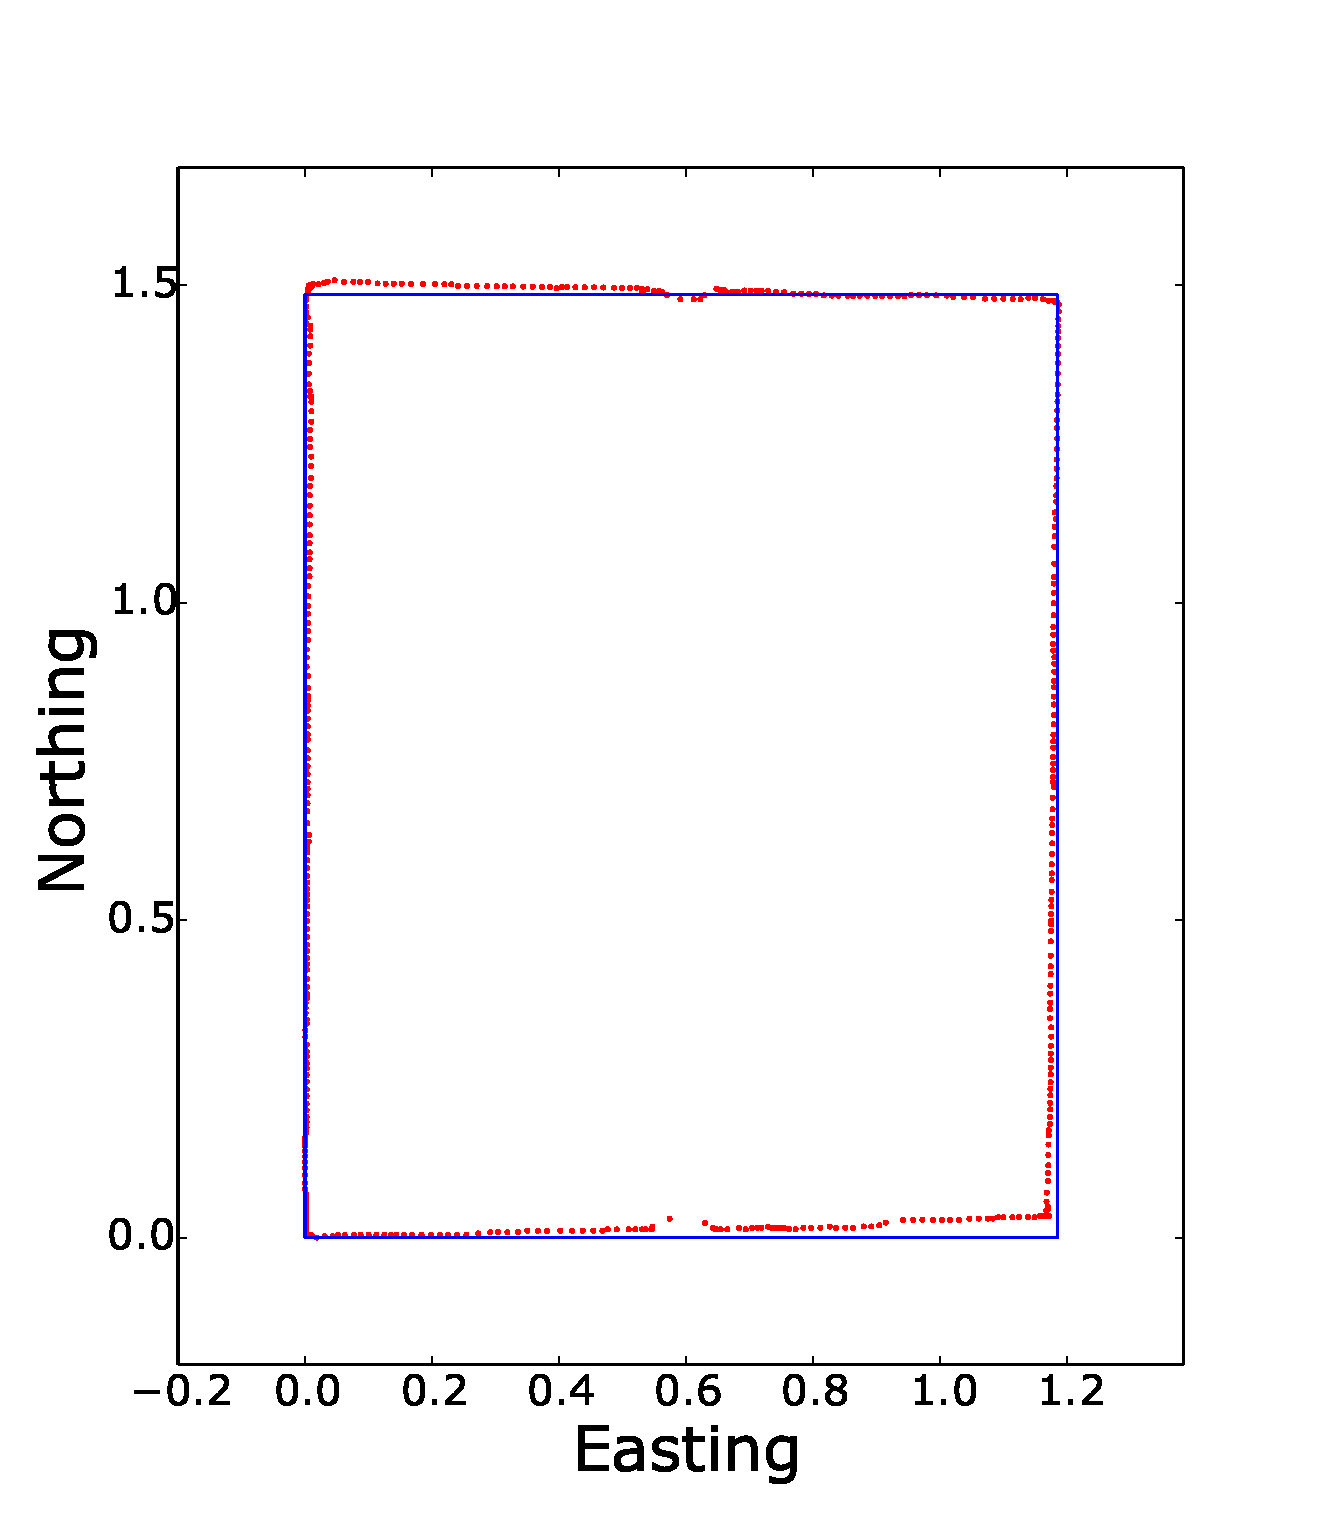
\includegraphics[width=\textwidth]{graphics/coordincate_conversion_test.eps}
        \caption{Blue 
rectangle is the whiteboard seen in figure \ref{fig:convert_test}. The red dots is output in \ac{LL} converted to UTM to be plotted}
        \label{fig:coordinate_test_polot}
    \end{subfigure}
    ~ %add desired spacing between images, e. g. ~, \quad, \qquad, \hfill etc. 
      %(or a blank line to force the subfigure onto a new line)
    \begin{subfigure}[b]{0.45\textwidth}
        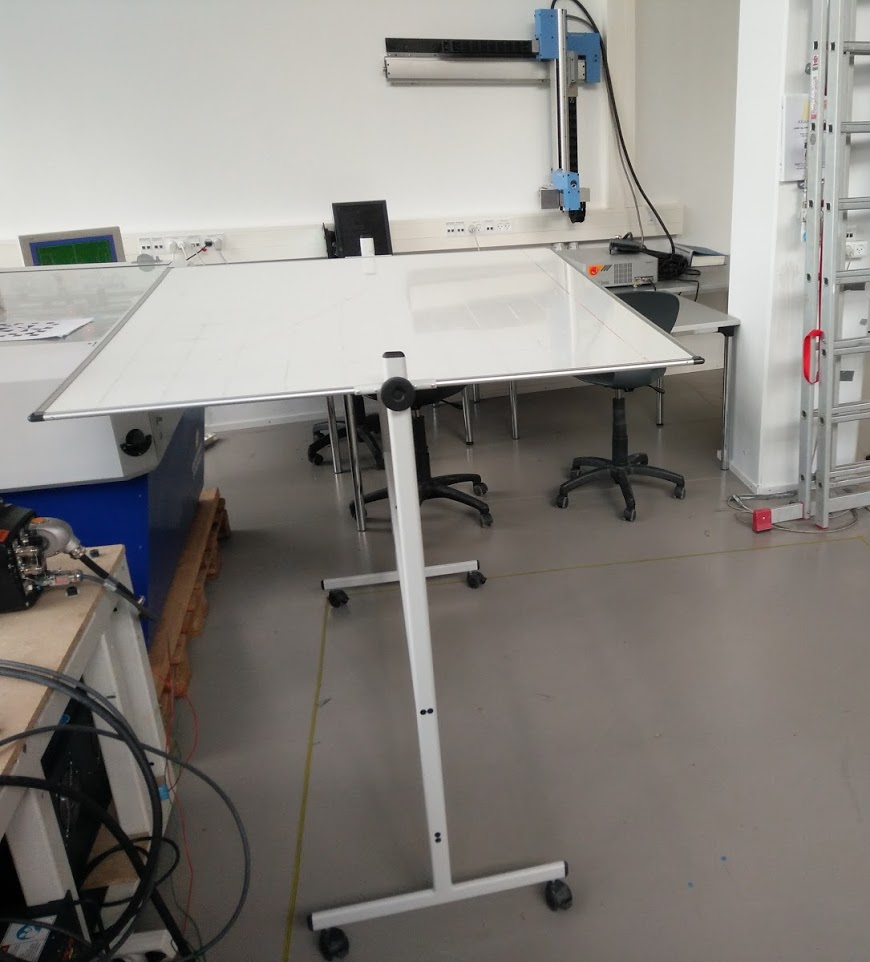
\includegraphics[width=0.95\textwidth]{graphics/coordinate_test_setup.png}
        \caption{A 4 order marker held along the edge of the whiteboard all the way around. The size of the whiteboard is 118.5cm*148.5 cm}
        \label{fig:convert_test}
    \end{subfigure}
\end{figure}

Figure \ref{fig:coordinate_test_polot} shows a blue 
rectangle representing the whiteboard shown in figure \ref{fig:convert_test}. The anomalies shown in the top and bottom of the 
rectangle is caused by the mountings holding the whiteboard. The software setup used to track the marker is shown in figure \ref{sec:indoor_localization}.
In this test, the \textit{Decision\_Maker} was programmed to let the output position be equal to the input position.
By doing this, it is possible to simply plot the position of the drone. Instead of transmitting the \ac{LL} frames to the drone they were logged and converted back to \ac{UTM} in order to be drawn together with the blue 
rectangle.
The lines were analyzed independently in order to see how well the fit a line. Since the whiteboards sides are straight lines, it was expected to see the marker moved along straight lines as well.


\begin{table}[H]
\centering
\caption{Results from positions obtaining by moving marker along the edge of whiteboard}
\label{tab:converter_results}
\begin{tabular}{@{}|l|l|l|@{}}
\toprule
\textbf{Side} & \textbf{Mean [M]}  & \textbf{Std. Deviation {[}M{]}} \\ \midrule
Left side     & 0.0040 & 0.0025                  \\ \midrule
Bottom side   & 0.014 & 0.01                   \\ \midrule
Right side    & 1.177 & 0.005                   \\ \midrule
Top side      & 1.490 & 0.009                   \\ \bottomrule
\end{tabular}
\end{table}

By calculating the different in means pairwise and subtract that from the actual size of the whiteboard, errors can be estimated.
The errors is 1.2 cm and 0.9 cm in width and height respectively.

The variance in table \ref{tab:converter_results} expresses how straight the marker has moved along the four sides. It can be seen that the variance is higher in top and bottom of the whiteboard, however this might be caused by the two mountings on the whiteboard causing some anomalies.
By inspection of \ref{fig:coordinate_test_polot} it can be seen how the red dots start to deviate from the blue lines at the upper-left and bottom-right corners. This indicates the marker was not moved precise enough at the two corners. However the results stated 


It can be concluded that creating a node being responsible of calculating the drones position in {LL} works. By moving a 4 order marker along a rectangle the size of the rectangle can be estimated with an error of 1.2 and 0.9 in with and height respectively. Due to lack of time, it was not possible to test if manipulating the drones position is adequate in order to control a drone.